\documentclass[norsk,a4paper,12pt]{beamer}
\usepackage[utf8]{inputenc}
\usepackage{graphicx} %for å inkludere grafikk
\usepackage{verbatim} %for å inkludere filer med tegn LaTeX ikke liker


\begin{document}
  \begin{frame}
    \frametitle{Coupled-Cluster teori}
    \framesubtitle{Fra Schrodingers ligning til dataprogram}
    Total bølgefunksjon:
    \begin{equation}
    |\Psi\rangle=e^{\hat{T}}|\Phi\rangle
    \end{equation}
  hvor $\Phi$ er referansebølgefunksjonen. 
    
  \end{frame}
  \begin{frame}
    \frametitle{Introduksjon}
    \framesubtitle{Slaterdeterminanten}
    Slaterdeterminanten for N partikler på Diracform
    \begin{equation}
    |\Phi\rangle=|\phi_i(x_1)\phi_j(x_2)\cdots\phi_o(x_N)\rangle
    \end{equation}
    Orbitalfunksjoner
    \begin{equation}
    f_i(x_m)=\sum_a t_i^a\phi_a(x_m),\quad f_{ij}(x_m,x_n)=\sum_{a>b}t_{ij}^{ab}\phi_a(x_m)\phi_b(x_n)
    \end{equation}
  \end{frame}
  \begin{frame}
    \frametitle{Introduksjon}
    \framesubtitle{Forbedret bølgefunksjon}
    \begin{figure}[h]
\centering
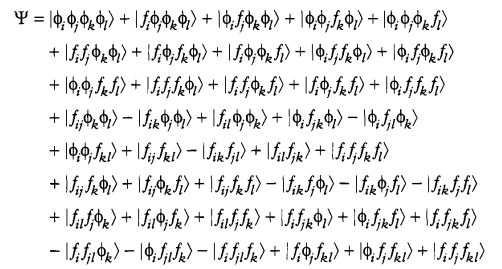
\includegraphics[width=100mm]{total_wf.png}
\end{figure}
  \end{frame}
  \begin{frame}
    \frametitle{Introduksjon}
    \framesubtitle{Orbitaloperatorer}
    \begin{equation}
    \hat{t}_i\equiv \sum_a t_i^a c_a^{\dagger}c_i,\quad \hat{t}_{ij}\equiv\sum_{a>b}t_{ij}^{ab}c_a^{\dagger}c_b^{\dagger}c_jc_i
    \end{equation}
    Som gir en total bølgefunksjon på 
    \begin{align*}
    |\Psi\rangle&=\bigg(1+\sum_i\hat{t}_i+\frac{1}{2}\sum_{ij}\hat{t}_i\hat{t}_j+\frac{1}{6}\sum_{ijk}\hat{t}_i\hat{t}_j\hat{t}_k\\
    &\mathrel{\phantom{=}}+\frac{1}{2}\sum_{ij}\hat{t}_{ij}
    +\frac{1}{8}\sum_{ijkl}\hat{t}_{ij}\hat{t}_{kl}+\frac{1}{24}\sum_{ijkl}\hat{t}_i\hat{t}_j\hat{t}_k\hat{t}_l\\
    &\mathrel{\phantom{=}}+\frac{1}{2}\sum_{ijk}\hat{t}_{ij}\hat{t}_k+\frac{1}{4}\sum_{ijkl}\hat{t}_{ij}\hat{t}_k\hat{t}_l\bigg)|\Phi\rangle
    \end{align*}
    
  \end{frame}
  \begin{frame}
    \frametitle{Introduksjon}
    \framesubtitle{Totale clusteroperatorer}
    \begin{align*}
    \hat{T}_1&=\sum_i\hat{t}_i=\sum_{ia}t_i^ac_a^{\dagger}c_i\\
    \hat{T}_2&=\frac{1}{2}\sum_{ij}\hat{t}_{ij}=\frac{1}{4}\sum_{ijab}\hat{t}_{ij}^{ab}c_a^{\dagger}c_b^{\dagger}c_jc_i
    \end{align*}
    som gir
    \begin{align*}
    |\Psi\rangle=\bigg(&1+\hat{T}_1+\frac{1}{2!}\hat{T}_1^2+\frac{1}{3!}\hat{T}_1^3+\hat{T}_2\\
    &+\frac{1}{2!}\hat{T}_2^2+\frac{1}{4!}\hat{T}_1^4+\hat{T}_2\hat{T}_1+\frac{1}{2!}\hat{T}_2\hat{T}_1^2\bigg)|\Phi\rangle
    \end{align*}
  \end{frame}
  \begin{frame}
    \frametitle{Introduksjon}
    \framesubtitle{Forenklet bølgerfunksjon}
    Vi definerer $\hat{T}\equiv\hat{T}_1+\hat{T}_2$:
    \begin{equation}
    |\Psi\rangle=e^{\hat{T}_1+\hat{T}_2}|\Phi\rangle\equiv e^{\hat{T}}|\Phi\rangle
    \end{equation}
    hvor
    \begin{equation}
    e^{\hat{T}}=1+\hat{T}+\frac{\hat{T}^2}{2!}+\frac{\hat{T}^3}{3!}+\sum_{n=4}^{\infty}\frac{\hat{T}^n}{n!}
    \end{equation}
  \end{frame}
  \begin{frame}
    \frametitle{Ulinkede CC ligninger}
    \framesubtitle{...}
    Energiligning
    \begin{equation}
    \langle\Phi|\hat{H}e^{\hat{T}}|\Phi\rangle=E
    \end{equation}
    Amplitudeligning
    \begin{equation}
    \langle\Phi_X|\hat{H}e^{\hat{T}}|\Phi\rangle=0.
    \end{equation}
    
  \end{frame}
  \begin{frame}
    \frametitle{Linkede CC ligninger}
    \framesubtitle{...}
    
    \begin{align}
    \langle\Phi|e^{-\hat{T}}\hat{H}e^{\hat{T}}|\Phi\rangle&=E\\
    \langle\Phi_X|e^{-\hat{T}}\hat{H}e^{\hat{T}}|\Phi\rangle&=0
    \end{align}

  \end{frame}
  \begin{frame}
    \frametitle{Å regne med de linkede CC ligningene}
    \framesubtitle{Hausdorffs ekspansjon}
    \begin{align*}
    e^{-\hat{T}}\hat{H}e^{\hat{T}}&=\hat{H}+[\hat{H},\hat{T}]+\frac{1}{2!}[[\hat{H},\hat{T}],\hat{T}]+\frac{1}{3!}[[[\hat{H},\hat{T}],\hat{T}],\hat{T}]+\cdots\\
    &=\hat{H}+\{\hat{H}\hat{T}\}_c+\frac{1}{2}\{\{\hat{H}\hat{T}\}_c\hat{T}\}_c+\hdots
    \end{align*}
  \end{frame}
  \begin{frame}
    \frametitle{Hamiltonianoperatoren}
    \framesubtitle{...}
    Hamiltonoperatoren
    \begin{equation*}
    \hat{H}=E_{ref}+\hat{F}_N+\hat{V}_N
    \end{equation*}
    med
    \begin{align*}
    \hat{F}_N=\sum_{pq}f_q^p\{c_p^{\dagger}c_q\},\quad \hat{V}_N=\frac{1}{4}\sum_{pqrs}W_{rs}^{pq}\{c_p^{\dagger}c_q^{\dagger}c_sc_r\}
    \end{align*}
    Vi vårt tilfelle får
    \begin{align*}
    e^{-\hat{T}}\hat{H}_Ne^{\hat{T}}&=\hat{H}_N+\{\hat{F}_N\hat{T}_1\}_c+\{\hat{V}_N\hat{T}_1\}_c+\{\hat{F}_N\hat{T}_2\}_c\\
    &\mathrel{\phantom{=}}+\{\hat{V}_N\hat{T}_2\}_c+\{\hat{F}_N\hat{T}_1^2\}_c+\{\hat{V}_N\hat{T}_1^2\}_c
    \end{align*}
  \end{frame}
  \begin{frame}
    \frametitle{Motivasjon}
    \framesubtitle{Matriseelementene i energiligningen}
    \begin{align*}
    \langle\Phi|\hat{H}_N|\Phi\rangle&=0\\
    \langle\Phi|\{\hat{F}_N\hat{T}_1\}_c|\Phi\rangle&=\sum_{ia}f_a^it_i^a\\
    \langle\Phi|\{\hat{V}_N\hat{T}_1\}_c|\Phi\rangle&=0\\
    \langle\Phi|\{\hat{F}_N\hat{T}_2\}_c|\Phi\rangle&=0\\
    \langle\Phi|\{\hat{V}_N\hat{T}_2\}_c|\Phi\rangle&=\frac{1}{4}\sum_{aibj}W_{ab}^{ij}t_{ij}^{ab}\\
    \frac{1}{2}\langle\Phi|\{\hat{F}_N\hat{T}_1^2\}_c|\Phi\rangle&=0\\
    \frac{1}{2}\langle\Phi|\{\hat{V}_N\hat{T}_1^2\}_c|\Phi\rangle&=\frac{1}{2}\sum_{aibj}W_{ab}^{ij}t_i^at_j^b
    \end{align*}
    
  \end{frame}
  \begin{frame}
    \frametitle{Motivasjon}
    \framesubtitle{Matriseelementene i amplitudeligningen}
    Nå har vi altså i prinsippet funnet et uttrykk for energien $E$ som en funksjon av amplitudene når vi antar at $f_q^p$ og $W_{ab}^{ij}$ er gitt. For å finne amplitudene, må vi først finne matriseelementene i amplitudeligningen. I motsetning til for energiligningen, skriver jeg bare opp de leddene som gir full kontraksjon og som dermed bidrar (ettersom vi får veldig mange ledd):
    \begin{align*}
    \langle\Phi_i^a|\hat{F}_N|\Phi\rangle&=\\
    \end{align*}
  \end{frame}
  \begin{frame}
    \frametitle{Motivasjon}
    \framesubtitle{...}
    
  \end{frame}
  \begin{frame}
    \frametitle{Motivasjon}
    \framesubtitle{...}
    
  \end{frame}
  \begin{frame}
    \frametitle{Motivasjon}
    \framesubtitle{...}
    
  \end{frame}
  \begin{frame}
    \frametitle{Motivasjon}
    \framesubtitle{...}
    
  \end{frame}
  
  
% etc
\end{document}